%
% hardware.tex
%
% Copyright (C) 2021 by SpaceLab.
%
% TTC 2.0 Documentation
%
% This work is licensed under the Creative Commons Attribution-ShareAlike 4.0
% International License. To view a copy of this license,
% visit http://creativecommons.org/licenses/by-sa/4.0/.
%

%
% \brief Hardware project chapter.
%
% \author Gabriel Mariano Marcelino <gabriel.mm8@gmail.com>
%
% \institution Universidade Federal de Santa Catarina (UFSC)
%
% \version 0.0.0
%
% \date 2021/04/02
%

\chapter{Hardware} \label{ch:hardware}

.

\begin{figure}[!h]
	\begin{center}
		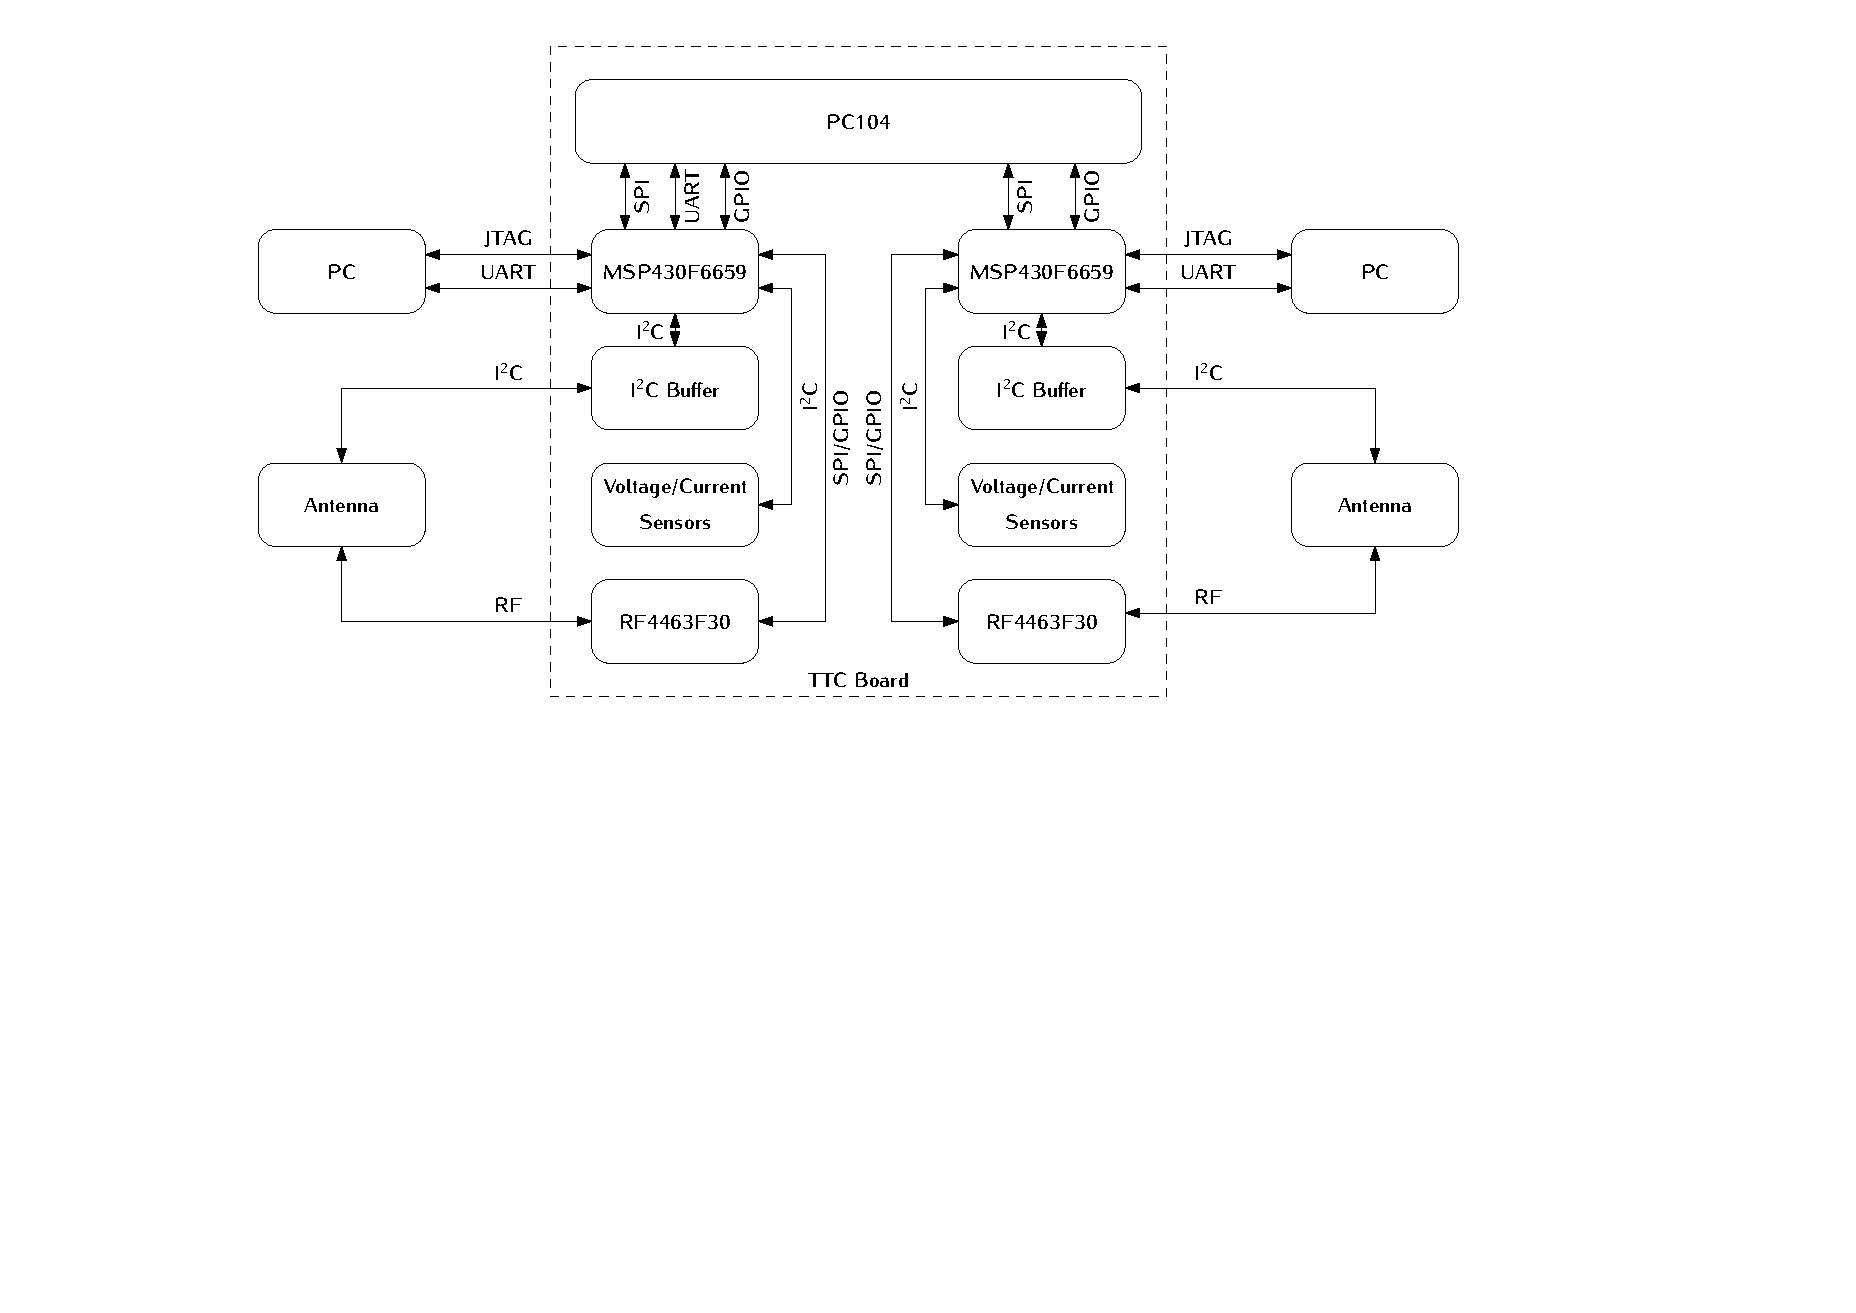
\includegraphics[width=\textwidth]{figures/hardware_diagram.pdf}
		\caption{Block diagram of the TTC 2 hardware.}
		\label{fig:hardware-diagram}
	\end{center}
\end{figure}

\section{PC-104}

The connector referred as PC-104 is a junction of two double row 26 pin headers (\textit{SSW-126-04-G-D}). These connectors create a solid 104-pin interconnection across the different satellite modules. \autoref{tab:pc104-pinout} provides the connector pinout\footnote{This pinout is simplified since additional interfaces were omitted. Refer to \textit{option sheet} in chapter \ref{ch:assembly}.} for the pins that are connected to the module. A reference of the pins' position can also be seen in \autoref{fig:pc104-ref-diagram}, a description of the signal is available in \autoref{tab:pc104-signals}.

\begin{figure}[!ht]
    \begin{center}
        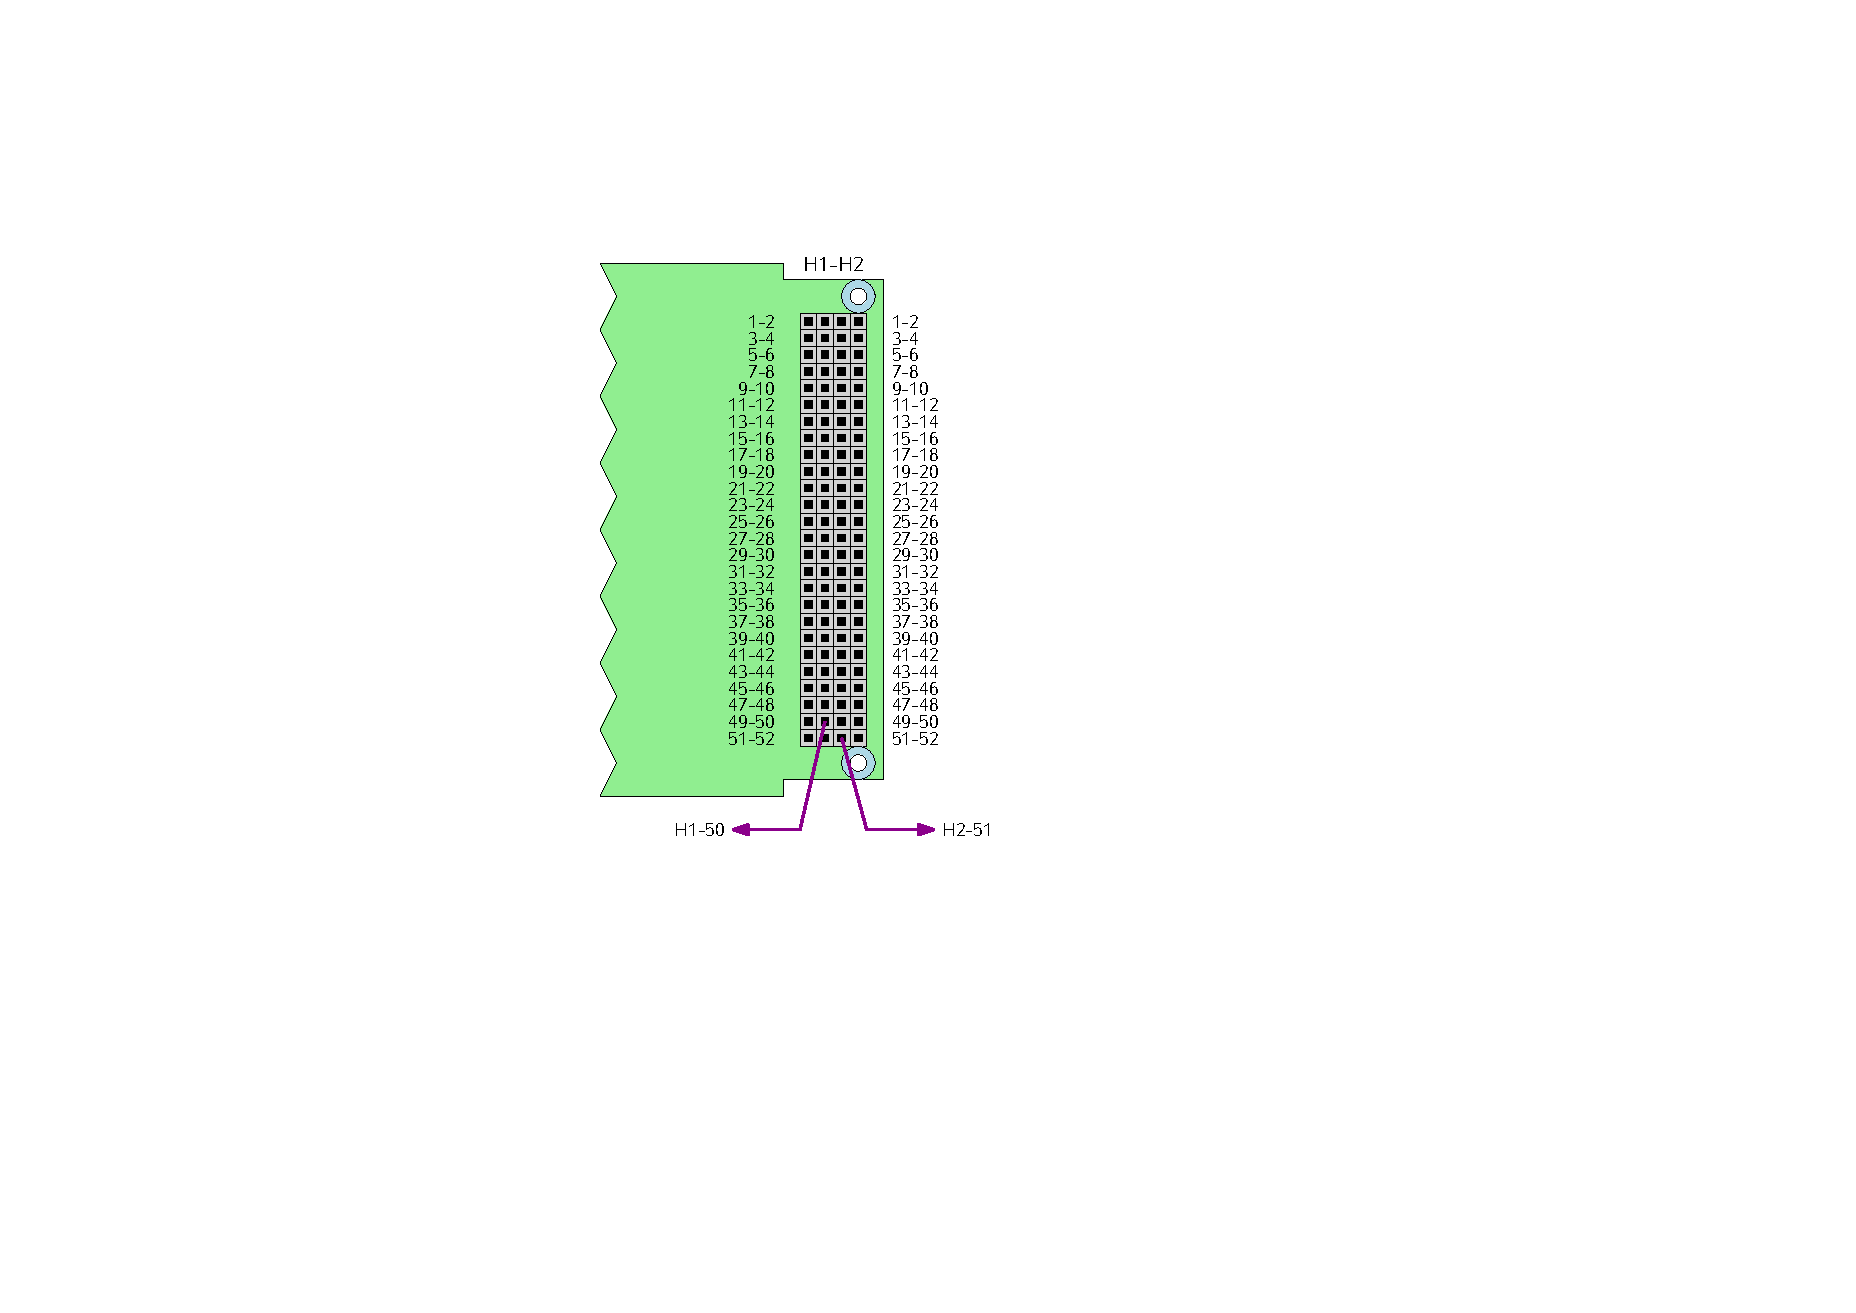
\includegraphics[width=0.5\textwidth]{figures/pc104-diagram}
        \caption{Reference diagram of the PC-104 bus (top view of a generic module).}
        \label{fig:pc104-ref-diagram}
    \end{center}
\end{figure}

\begin{table}[!h]
    \centering
    \begin{tabular}{cllll}
        \toprule[1.5pt]
        \textbf{Pin Row}   & \textbf{H1 Odd}  & \textbf{H1 Even} & \textbf{H2 Odd}  & \textbf{H2 Even} \\
        \midrule
        1-2                & -                & -                & -                & -                \\
        3-4                & -                & -                & -                & -                \\
        5-6                & -                & -                & RA\_1\_UART\_RX  & -                \\
        7-8                & GPIO\_6          & GPIO\_7          & RA\_1\_UART\_TX  & GPIO\_0          \\
        9-10               & RA\_1\_SPI\_INT  & RA\_1\_EN        & -                & -                \\
        11-12              & RA\_0\_SPI\_INT  & RA\_0\_EN        & RA\_1\_SPI\_MOSI & RA\_1\_SPI\_CLK  \\
        13-14              & -                & -                & RA\_1\_SPI\_CS   & RA\_1\_SPI\_MISO \\
        15-16              & -                & -                & -                & -                \\
        17-18              & -                & -                & -                & GPIO\_1          \\
        19-20              & -                & GPIO\_2          & -                & GPIO\_3          \\
        21-22              & -                & -                & -                & GPIO\_4          \\
        23-24              & -                & -                & -                & -                \\
        25-26              & -                & -                & -                & -                \\
        27-28              & -                & -                & VCC\_3V3         & VCC\_3V3         \\
        29-30              & GND              & GND              & GND              & GND              \\
        31-32              & GND              & GND              & GND              & GND              \\
        33-34              & -                & -                & -                & -                \\
        35-36              & RA\_0\_SPI\_CLK  & -                & VCC\_3V3\_ANT    & VCC\_3V3\_ANT    \\
        37-38              & RA\_0\_SPI\_MISO & -                & -                & -                \\
        39-40              & RA\_0\_SPI\_MOSI & RA\_0\_SPI\_CS   & -                & -                \\
        41-42              & -                & -                & -                & GPIO\_5          \\
        43-44              & -                & -                & -                & -                \\
        45-46              & -                & -                & -                & -                \\
        47-48              & -                & -                & -                & -                \\
        49-50              & VCC\_5V\_RA\_0   & VCC\_5V\_RA\_0   & -                & -                \\
        51-52              & VCC\_6V\_RA\_1   & VCC\_6V\_RA\_1   & -                & -                \\
        \bottomrule[1.5pt]
    \end{tabular}
    \caption{PC-104 bus pinout.}
    \label{tab:pc104-pinout}
\end{table}

\begin{table}[!h]
    \centering
    \begin{tabular}{lL{0.3\textwidth}l}
        \toprule[1.5pt]
        \textbf{Signal}  & \textbf{Pin(s)}                  & \textbf{Description} \\
        \midrule
        GND              & H1-29/30/31/32, H2-29/30/31/32   & Ground reference                      \\
        VCC\_3V3         & H2-27, H2-28                     & TTC power supply (3,3 V)              \\
        VCC\_3V3\_ANT    & H2-35, H2-36                     & Antenna power supply (3,3 V)          \\
        VCC\_5V\_RA\_0   & H1-49, H1-50                     & Radio 0 power supply (5 V)            \\
        VCC\_6V\_RA\_1   & H1-51, H1-52                     & Radio 1 power supply (6 V)            \\
        RA\_0\_SPI\_CLK  & H1-35                            & CLK signal of the radio 0 SPI bus     \\
        RA\_0\_SPI\_MISO & H1-37                            & MISO signal of the radio 0 SPI bus    \\
        RA\_0\_SPI\_MOSI & H1-39                            & MOSI signal of the radio 0 SPI bus    \\
        RA\_0\_SPI\_CS   & H1-40                            & CS signal of the radio 0 SPI bus      \\
        RA\_0\_SPI\_INT  & H1-11                            & INT signal of the radio 0 SPI bus     \\
        RA\_1\_SPI\_CLK  & H2-12                            & CLK signal of the radio 0 SPI bus     \\
        RA\_1\_SPI\_MISO & H2-14                            & MISO signal of the radio 0 SPI bus    \\
        RA\_1\_SPI\_MOSI & H2-11                            & MOSI signal of the radio 0 SPI bus    \\
        RA\_1\_SPI\_CS   & H1-13                            & CS signal of the radio 0 SPI bus      \\
        RA\_1\_SPI\_INT  & H1-9                             & INT signal of the radio 0 SPI bus     \\
        RA\_1\_UART\_RX  & H2-5                             & RX signal of the radio 1 UART         \\
        RA\_1\_UART\_TX  & H2-7                             & TX signal of the radio 1 UART         \\
        RA\_0\_EN        & H1-11                            & Radio 0 power enable                  \\
        RA\_1\_EN        & H1-9                             & Radio 1 power enable                  \\
        GPIO\_N          & H1-7/8/19, H2-8/18/20/22/42      & GPIO pin (not used)                   \\
        \bottomrule[1.5pt]
    \end{tabular}
    \caption{PC-104 bus signal description.}
    \label{tab:pc104-signals}
\end{table}

The distribution pattern of pins adopted in this project is a mix of multiple different patterns from CubeSat modules manufacturers, like GomSpace, ISIS and Endurosat. Some pins are positioned to attend specific project requirements, and it is possible that the adopted pattern is not totally compatible to some commercial modules.
